\documentclass[12pt,a4paper]{article}
\usepackage{ucs}
\usepackage{caption}
\usepackage[latin1,utf8x]{inputenc}
\usepackage{amsmath}
\usepackage{caption}
\captionsetup{font=small,labelfont=bf}
\usepackage[danish]{babel}
\usepackage[rmargin=3cm,tmargin=3.3cm]{geometry}
\usepackage{listings}
\usepackage{color}
\setlength{\parindent}{0pt}
\setlength{\parskip}{1ex plus 0.5ex minus 0.2ex}
\usepackage{graphicx}
\usepackage{fixltx2e}

\usepackage[T1]{fontenc}
\usepackage{textcomp}


%insert links
\usepackage{hyperref}
\usepackage{fancyhdr,lastpage}	
\pagestyle{fancy}


\definecolor{mygreen}{rgb}{0,0.6,0}
\definecolor{myblue}{rgb}{0,0,1}
\definecolor{myyellow}{rgb}{0.7,0.7,0}
\definecolor{myblack}{rgb}{0,0,0}

\lstset{
	breaklines=true,
	numbers=left, 
	commentstyle=\color{mygreen},
	stringstyle=\color{myyellow},
}

%header
\lhead{ 
	Embedded Systems \\
	02131 \\ 
}
\chead{ 
}
\rhead{ 2 October, 2012 \\ \bigskip  }

%Footer
\lfoot{
	\rule{\textwidth}{0.1mm}\\
}

\cfoot{}
\rfoot{\ \\ \scriptsize{Side \thepage\ af \pageref{LastPage}}}

\begin{document}

%Forside
\begin{titlepage}
	\begin{center}
		\vspace*{13\baselineskip}
		\huge
		\bfseries
		Embedded Systems\\ 
		\ \\
		02131 \\[5\baselineskip]

		\normalfont
		\Large
		R-peak detection!\\	
		2013

		\small
		\vfill
	\end{center}	
	\begin{flushleft}
		Jakob Welner, s124305\\
	 	Jacob Gjerstruo, s113440\\
	\end{flushleft}
\end{titlepage}

\ \\
\section*{Abstract}
The task of this assignment was to show by proof-of-concept that a dedicated processor could be created through the Gezel hardware description language. This dedicated processor was created in such a way that it could accept the assembly code that had manually been translated from the C-code of the MWI filter. Once this assembly code had been read, it would then be able to calculate the data, as determined by the filter. This dedicated processor were then attached to a bus, the data were migrated away from the processor itself into a seperate module which was also connected to the bus, and a protocol for these were developed.

\thispagestyle{empty} 
\newpage

%Table of Contents
\tableofcontents
\thispagestyle{empty} 
\newpage

%Reset pagecount
\setcounter{page}{1}

%Alm. sider
\ \\
\section{Introduction}
	After successfully proving in assignment 1 that the QRS algorithm could be implemented, Medembed now wants a proof of concept that this QRS algorithm can be implemented by using a small embedded processor. To do this, one of the filters will be implemented through the use of the Hardware Description Language (HDL) Gezel.\\
	This report will discuss how the filter will be implemented through Gezel, as well as the following topics: Modules of the processor, Instruction set for the processor, Controller for the processor, Integration of the processor into a combined system, and finally, the critical parts of the processor, i.e. speed (clock cycles per second), power consumption (watt) and size (memory requirements).\\
	For the purpose of this report, the data for the filter will be loaded through a file one data point at a time and then be processed by our simulated hardware.\\
	
\subsection{Requirements}
Below follows a list of functional and non-functional requirements:\\

\textbf{ Functional requirements for the application:}
\begin{itemize}
	\item Each module of the processor must first be built, run and tested by their own
	\item An instruction set must be designed
	\item A controller for the instruction set must be designed
	\item The controller must be integrated into a larger system
	\item The performance of the system must be analysed in terms of speed and memory requirements

\end{itemize}
\textbf{Non-functional requirements for the application:}
\begin {itemize}
	\item The processor must be implemented with the use of Gezel
\end{itemize}

\section{Analysis}
 	In order to initiate the structure- and design-process of the program, a number of questions needed to be answered first:\\
 	
 	\begin{enumerate}
	\item How could the C-code be compiled into hardware instructions
	\item Which instructions would be needed to accomplish this?
	\item Which hardware modules would be needed to execute the instructions?	
	\item How could the CPU be designed in order to understand the instruction set?
	\item How could the CPU be integrated into a system?
	\item What would the critical parts of the system be and how could these be analysed?
\end{enumerate}

\subsection{Problem 1: Hardware modules}
	To gain a basic understanding of GEZEL and hardware design, an initial guide was given that suggested the creation of the following modules, as well as how to make these: Counter, Adder, Multiplexer, Arithmetic Logic Unit (ALU) with and without status flags, a register file and an instruction memory block. Each module was written and verified by running them through a testbench.\\
\subsection{Problem 2: Instruction set}
	Designing the instruction set was a fairly arbitrary task, as there were very few limitations and the instructions in theory could be anything.
The first question here was whether the instructions should be able to execute on single cycles or be more complex and execute across several cycles (RISC vs. CISC). The former (RISC) was chosen as a basis for the instruction set. A theoretical assembly code was made based on the assumption of single-clock instructions, where instructions were added to the list as they became needed. From this theoretical assembly code the instruction set was extracted.\\
	
\subsection{Problem 3: Implementation of the CPU}
	Once the instruction set was finished, the next part would be to implement a CPU that could understand and execute the instruction set. To do this, a block diagram was to be designed to get an overview of how each component should be connected.\\
	Once the block diagram was completed and all components were connected, the next issue became to distinguish control- and data signals - here, control signals configure a single component whereas data signals carry data between the components. This would be the second issue of implementing the controller - which are the control signals and which are the data signals and how can these be implemented?\\
	
\subsection{Problem 4: System Integration}
	With the controller done, the next step is to integrate the processor into the system. To do this, the controller must be connected to a bus which uses a master/slave protocol - here, the processor is the master. The protocol between the master and the slave has already been defined, and so, the only real issues were how to ensure that when the master sends data to the slave, the slave will always respond with data, as well as making sure the slave can analyse the commands from the processor correctly and carry out the correct instruction on the data.\\
	
\subsection{Problem 5: Critical parts}
	There are three terms that needs to be discussed when it comes to the critical parts of the processor: Size, speed and power.\\
	The speed of the processor is the most important of these up to a certain threshold, as it needs to be capable of making the computation of the 250 data points per second and display the result to the user. However, once this threshold has been reached, the speed becomes the least most important part, as it will merely have to idle after this threshold, spending power on nothing.\\
	Power and size are equally important, as the bigger the processor is, the more cumbersome the ECG scanner will be for a user to wear, and the more power it consumes, the more often it will need to be recharged or have the battery replaced. Therefore, the three problems becomes:
	
	\begin{itemize}
		\item Is the processor fast enough, and if it is, how much idle time is there between data points?
		\item What is the memory consumption of the processor and what can be done to reduce this?
		\item How much energy does the processor consume and what can be done to reduce that?
	\end{itemize}
	
\section{Implementation}
\subsection{Processor modules}
	To implement each module, we quickly decided that for the lone implementation of these, it was most optimal to implement each with a testbench to test various cases. The code for these modules as well as their testbenches can be seen in the appendix.\\
	Regarding whether we needed all modules for this processor, it was decided to implement all of them nevertheless in case we did need all modules.\\
	
\subsection{Instruction set}
	To ensure the processor could understand the instruction set, it was decided to do this in assembly code, as this is a very low level programming language that is universally used when writing directly to a processor.\\
	Once that decision had been taken, it was time to convert the C code manually into instructions in assembly code. The first thing that was done was to design the actual instructions set - this set would be the commmands used in the actual instructions, and for this processor, it consists of 11 different commands:\\
	
	\begin{itemize}
			
			\item LOAD R0 X: Loads a value (line number X) and stores it into a variable (R0).
			\item STRE X R0: Stores the value of X in R0.
			\item MOVE R0 R1: Reads the value of R1 and stores it in R0.
			\item ADD R0 R1 R2: Adds two variables (R1 and R2) and stores it into a third one (R0).
			\item SUB R0 R1 R2: Subtracts two variables (R2 from R1; R1-R2) and stores it into a third one (R0).
			
			\item ADDI R0 R1 X: Add Immediate - it adds the value of X to the value of R1 and stores it in R0.
			\item SUBI R0 R1 X: Sub Immediate - it subtracts the value of x from R1 (R1-X) and stores in R0.
			\item SHRI R0 R1 X: Bitshift Right Immediate - bitshifts R1 right with the value of X and stores the result in R0.
			\item MULI R0 R1 R2: Multiplies R1 with R2 and stores in R0.
			\item BLILT R0 R1 X: Branch If Larger Than: Branches if R0 is larger than R1 and moves the scanner to line X.
			\item BRCH X: Returns the scanner of the code to line X.
		\end{itemize}
	The full instruction set can be seen in the appendix - in total, the instructions used are 17 lines long with the 11 different instructions written above.
\subsection{Implementation of the controller}
	aw
\subsection{System Integration}
	
\subsection{Critical parts}
	As was stated in the analysis, the critical parts involve three different things to be measured: Speed, size and power.\\
	Speed is measured in clock cycles, and for this program, there were 11 instructions. Of these 11 instructions, 8 takes 1 clock cycle, 1 takes 2 clock cycles (BRCH), and the last two takes 8 and 9 clock cycles, respectively (LOAD and STRE). For each data point after the 30'th, the program will carry out these instructions such that in total, each data point requires an estimated 29 clock cycles. Furthermore, the processor had to be able to handle 250 data points per second. With this knowledge, it's possible to calculate the number of clock cycles the processor MUST be able to handle per second, which is $29*250=7250$ clock cycles per second, after the 30'th data sample. This may initially seem like a high amount of cycles, but when compared to the fact that a standard, all-purpose processor like the Core I5 (which is a mid-range processor introduced in 2009 by Intel and used in many computers nowadays) runs at 2.7 GHz for the lowest, which is equivalent to 2.700.000.000 clock cycles per second, 7250 cycles does not seem like much and should be easily accomplished by the processor developed here.\\
	It should be noted here that clock cycles does not have any defined period, and some clock cycles are faster than other (for instance, 1 multiplication followed by a division could take 10ns, whereas 2 additions and an \& might only take 6ns). Therefore, to get a completely accurate view of this, it would be necessary to test how long the program actually takes to calculate these 250 data points, and then subsequently divide this number by 7250 (as this is the amount of clock cycles it should've taken). This would then give an average clock period per cycle.\\
	A guestimate on the optimal clock speed of our processor would therefore be around 15 KHz, which should be more than enough to calculate the necessary 250 data points per second and still have plenty of clock cycles to spare, should some of the clock cycles take drastically longer than others.\\
	\\
	In terms of size, this program has not been optimized for size - first and foremost, the importance was to ensure the program ran correctly and that it ran fast enough to accomplish the necessary the required 250 data points per second. To optimize for size, many of the data signals have been implemented with 32 bit registers of which many does not use all of the 32 bits - these could be scaled down to more reasonable values, depending on the signal.\\
	\\
	Finally, in terms of power, the main thing to look at would be to look at the number of signals that switches value, also called toggles. Gezel has a built in option to analyse this, and a screenshot of this can be seen below (the full toggle report can be seen here: \ref{toggle_full}):\\
	\begin{figure}[h!]
		\centering
			\includegraphics[width=1\textwidth]{Screenshots/Screenshot_profiling.png}
		\caption{A screenshot of the output of the toggle profiling result.}
		\label{toggle}
	\end{figure}
	
	What can be seen on figure \ref{toggle} is a list of cycles, their evaluations, the number of toggles and the values of all signals, be they 0 or 1. The interesting thing here is to look at the amount of toggles per cycle, as this is what can be optimized, so to figure out where to optimize the program in terms of power, the whole simulation is profiled with toggling, the cycles with the largest amount of toggles is then identified, and then the programmer needs to identify what happens in these cycles and then optimize this part.\\


\section{Results}
	
%	\begin{figure}[h!]
%		\centering
%			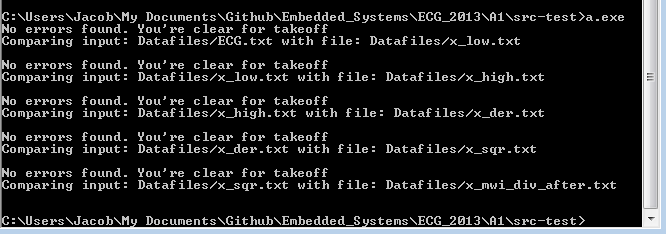
\includegraphics[width=1\textwidth]{Screenshots/tests_filter_result.png}
%		\caption{A screenshot of the output of the tests of the filters.}
%		\label{test_filter_result}
%	\end{figure}

\section{Design}
One of the more important design decisions when designing this processor was how to divide. This is not a simple thing to do in the hardware domain, and as a result, doing the division by 30 that the filter required a manual implementation. To handle this, a python script was created that would determine how to obtain the best approximation, and the end result was that an approximation gained by multiplying by 4369 and subsequently bitshifting by 17, both of which are simple operations already implemented in Gezel, would give 300 out of 10.000 data points where they would be 1 off their original value. This was found to be acceptable, as the values the processor operates on are in the several hundreds, meaning that the approximation are off by less than 1\%, and in most cases even off by less than one \textperthousand. Furthermore, it should be noted that the data are already rounded off by the fact that they are integers, and as such, it can be the approximation is actually closer to the correct value, compared to the value that was rounded off.\\
\\
Furthermore, it was decided that, rather than make a loop that would run through backwards and gather the 30 data points, the processor would instead simply hold an accumulation of the last 30 values. To this, it would add the next data point and subtract the point that was 30 points old and then subsequently multiply and bitshift - this should give a dramatical increase in calculation speed, as it no longer needs to loop back 30 data points and load all these before it multiplies and bitshifts. The benefit of this is that instead of making 30 additions and one division, the program need only make one addition, one subtraction and one division, which will increase the speed at which the algorithm runs. The negatives of this, though, is that the curve will have a ``soft'' start and will only work correctly after 30 data points.\\
\\
It was also decided that a new register had to be implemented in the decoder. The value of instVal would be stored in this register, and then read in the following clock cycle. The reason that this was necessary was that, due to the way Gezel is implemented, the signal of instVal would arrive a clock cycle earlier than its corresponding control signal. This workaround is not optimal, but it means that the program works as expected.\\
In the same way as above, another workaround was created around the fact that the ipblock will read an extra line whenever a jump command is sent before actually jumping. The workaround implemented here was to make a NoOPeration (NOP) after each jump, which wastes a cycle but ensures that the program calculates correctly after a jump command.\\
\\

\subsection{Improvements}
To improve on the design, changing the value of the MWI filter to sum over and divide by 32 would make both the implementation, maintenance and all the calculations involved much simpler (and thereby possibly also much faster) in that, instead of having to bitshift and multiply with 1.xxxxxxx, it would be possible to simply bitshift with 6 and that would be it, no further calculations would be necessary. Doing this would not include more additions either, thanks to the way that the summation has been implemented - all that should be changed would be to change the reference of how many steps back the program should go before subtracting. This goes beyond the scope of this report, though.\\
\\
A further improvement could be to do the addition and the subtraction in on cycle by combining the commands. This would spare one clock cycle per run of all the commands.\\
\\
The final improvement that this report has been able to identify would be to optimize the signal width; according to the data used in this report, no point is larger than 10.000, which means that no signal needs be larger than 14 bit, and thus could be reduced quite alot - to take into account, they could be reduced to a bitwidth of about 16 and still be within the limits of the data provided.\\

\section{Conclusion}
It has now been successfully demonstrated that it is possible to implement a dedicated processor for the task of calculating the data of the Mowing Window Integration filter. Furthermore, the critical parts of the processor has been analysed, and the speed of the processor has been determined, along with a way to optimize it in terms of both size and power.
\newpage
\begin{thebibliography}{9}

\bibitem{lamport94}
  Michael Reibel Boesen, Jan Madsen, Linas Kaminskas, Paul Pop, Karsten Juul Frederiksen\\
  \emph{Assignment 2: The ECG processor}\\
  2013.\\

\bibitem{Gezel}
  \emph{Lecture7: Finite state machine with Datapath}\\
  Fall, 2007.\\

\bibitem{GezelBasicSyntax}
  \emph{GEZEL Basic Syntax}\\
  
\bibitem{ClockSpeeds}
  \emph{http://smallbusiness.chron.com/ghz-mean-computer-processor-66857.html}
  Used to explain clock speeds of a processor
  
\bibitem{CoreI5}
  \emph{http://www.intel.com/content/www/us/en/processors/core/core-i5-processor.html}
  Used to determine clock speeds of Core I5
\end{thebibliography}
	
\newpage	
	\begin{Large}
		\textbf{Appendix}
	\end{Large}
	\appendix

\section{Who wrote what}
Jacob Gjerstrup, s113440 wrote: Introduction, Analysis (Problem 1, 2 and 5), Implementation (Processor, Instruction set, Critical Parts), Design\\
Jakob Welner, s124305 wrote: Abstract, Analysis (Problem 3+4), Implementation (Implementation of the Controller, System Integration), Design (Improvements section), Conclusion\\

\section{Sourcecode}

\subsection{Source code for the Processer modules}
	\subsubsection{Counter}
		\lstinputlisting[language=C]{Code/Proc_Mods/counter.fdl}	
	\subsubsection{Adder with testbench}
		\lstinputlisting[language=C]{Code/Proc_Mods/adder.fdl}	
	\subsubsection{Multiplexer}
		\lstinputlisting[language=C]{Code/Proc_Mods/mux.fdl}	
	\subsubsection{Arithmetic Logic Unit (ALU)}
		\lstinputlisting[language=C]{Code/Proc_Mods/ALU.fdl}
	\subsubsection{ALU with flags}
		\lstinputlisting[language=C]{Code/Proc_Mods/ALU_withFlags.fdl}	
	\subsubsection{Register}
		\lstinputlisting[language=C]{Code/Proc_Mods/register.fdl}	
	\subsubsection{Instruction Memory}
		\lstinputlisting[language=C]{Code/Proc_Mods/memory.fdl}	
\subsection{Instruction set}
	\lstinputlisting[language=C]{Code/assembly_mwint.asm}	
\subsection{Controller}
\subsection{Platform}
	\lstinputlisting[language=C]{Code/Platform.fdl}	
\subsection{Profiling}
	\label{toggle_full}	
	\lstinputlisting[language=C]{Code/toggle_output.txt}

\end{document}